\documentclass{report}

\usepackage{geometry}
\usepackage{amsmath}
\usepackage{graphicx}
\usepackage{url}

\renewcommand{\bibname}{References}

\graphicspath{ {./images/} }

\title{Furuta Pendulum Control Project Report}

\author{Samvrit Srinivas}

\date{\today}

\begin{document}

\maketitle

\chapter{Motor Controller} \label{chap:motor_controller}

The input for the furuta pendulum is a torque applied by the motor at the base of the setup. The high-level controller computes the amount of torque to be applied by the motor, and the low-level controller runs a PI control on the torque reference. We use a DC brushed motor for this purpose, and hence the motor controller is designed to be a current controller, as the torque is directly proportional to the winding current. The winding current is controlled by applying a pulse-width-modulated voltage at the motor terminals. In the following sections, we will look into the mathematical model and the control design of the current/torque controller.

\section{Motor Selection and Parameter Derivation}	\label{sec:motor_selection}
By simulating the high level controller with slightly different initial conditions, we were able to get an idea of the torque and speed requirements of the DC motor. A motor with a stall-torque rating of at least 4 Nm and a speed rating of at least 60 RPM was deemed necessary. A motor from Pololu was selected with the nameplate specifications shown in Table \ref{table:pololu_specs} \cite{pololu_motor_specs}.


\begin{table}
\begin{center}
\begin{tabular}{|c|c|}
\hline
\textbf{Parameter} & \textbf{Value }\\
\hline\hline
Voltage & 12V \\
\hline
No-load speed & 67 RPM \\
\hline
No-load current & 0.2 A \\
\hline
Stall torque & 4.9 Nm \\
\hline
Stall current & 5.5 A \\
\hline
\end{tabular}
\caption{Pololu motor nameplate specifications} \label{table:pololu_specs}
\end{center}
\end{table}


From the nameplate specifications and from CAD drawings provided by the manufacturer, the other motor parameters were derived, as shown in Table \ref{table:pololu_motor_params}.


\begin{table}
\begin{center}
\begin{tabular}{|c|c|c|}
\hline
\textbf{Parameter} & \textbf{Value} & \textbf{Units} \\
\hline \hline
$K_t$ & $0.968$ & $Nm/A$ \\
\hline
$K_v$ & $1.7103$ & $V/rad/s$ \\
\hline
$L$ & $2.3e-3$ & $H$ \\
\hline
$R$ & $2.18$ & $\Omega$ \\
\hline
$J$ & $12e-9$ & $kgm^2$ \\
\hline
$b$ & $0.0151$ & $Nm/rad/s$ \\
\hline
\end{tabular}
\caption{Motor parameters} \label{table:pololu_motor_params}
\end{center}
\end{table}

\subsection{Parameter Derivations}

\subsubsection{Torque Constant ($K_t$)}
\begin{equation}
K_t = \frac{\text{stall-torque}}{\text{stall-current}}
\end{equation}

\subsubsection{Back-EMF Constant ($K_v$)}
\begin{equation}
K_v = \frac{\text{nameplate voltage}}{\text{nameplate speed}}
\end{equation}

\subsubsection{Winding Inductance ($L$) and Resistance ($R$)}
\begin{equation}
R = \frac{\text{nameplate voltage}}{\text{stall current}}
\end{equation}
The inductance was provided by the manufacturer. It is also possible to measure the inductance using an LCR meter.

\subsubsection{Rotor Inertia ($J$)}
From the CAD model, the dimensions (volume and length) of the rotor were obtained. Assuming that the rotor is made of stainless steel, and using the density for stainless steel as $\rho = 7,500 kg/m^3$, the mass was determined. Using mass and length, the rotor inertia was estimated using
\begin{equation}
J = \frac{1}{12} \cdot m \cdot l^2
\end{equation}

\subsubsection{Coefficient of Viscous Friction ($b$)}
\begin{equation}
b = \frac{\text{no-load-current} \cdot K_t}{\text{no-load-speed}}
\end{equation}




\section{Mathematical Model of DC Motor}	\label{sec:math_model}

Since the winding current is controlled by applying a certain voltage at the motor terminals, it is beneficial to look at the transfer function $\frac{I(s)}{V(s)}$. Figure \ref{fig:dc_motor_transfer_fn} represents the current-voltage dynamics of a DC motor \cite{motor_control_umich_lecture}:\\

\begin{figure}[h]
\centering
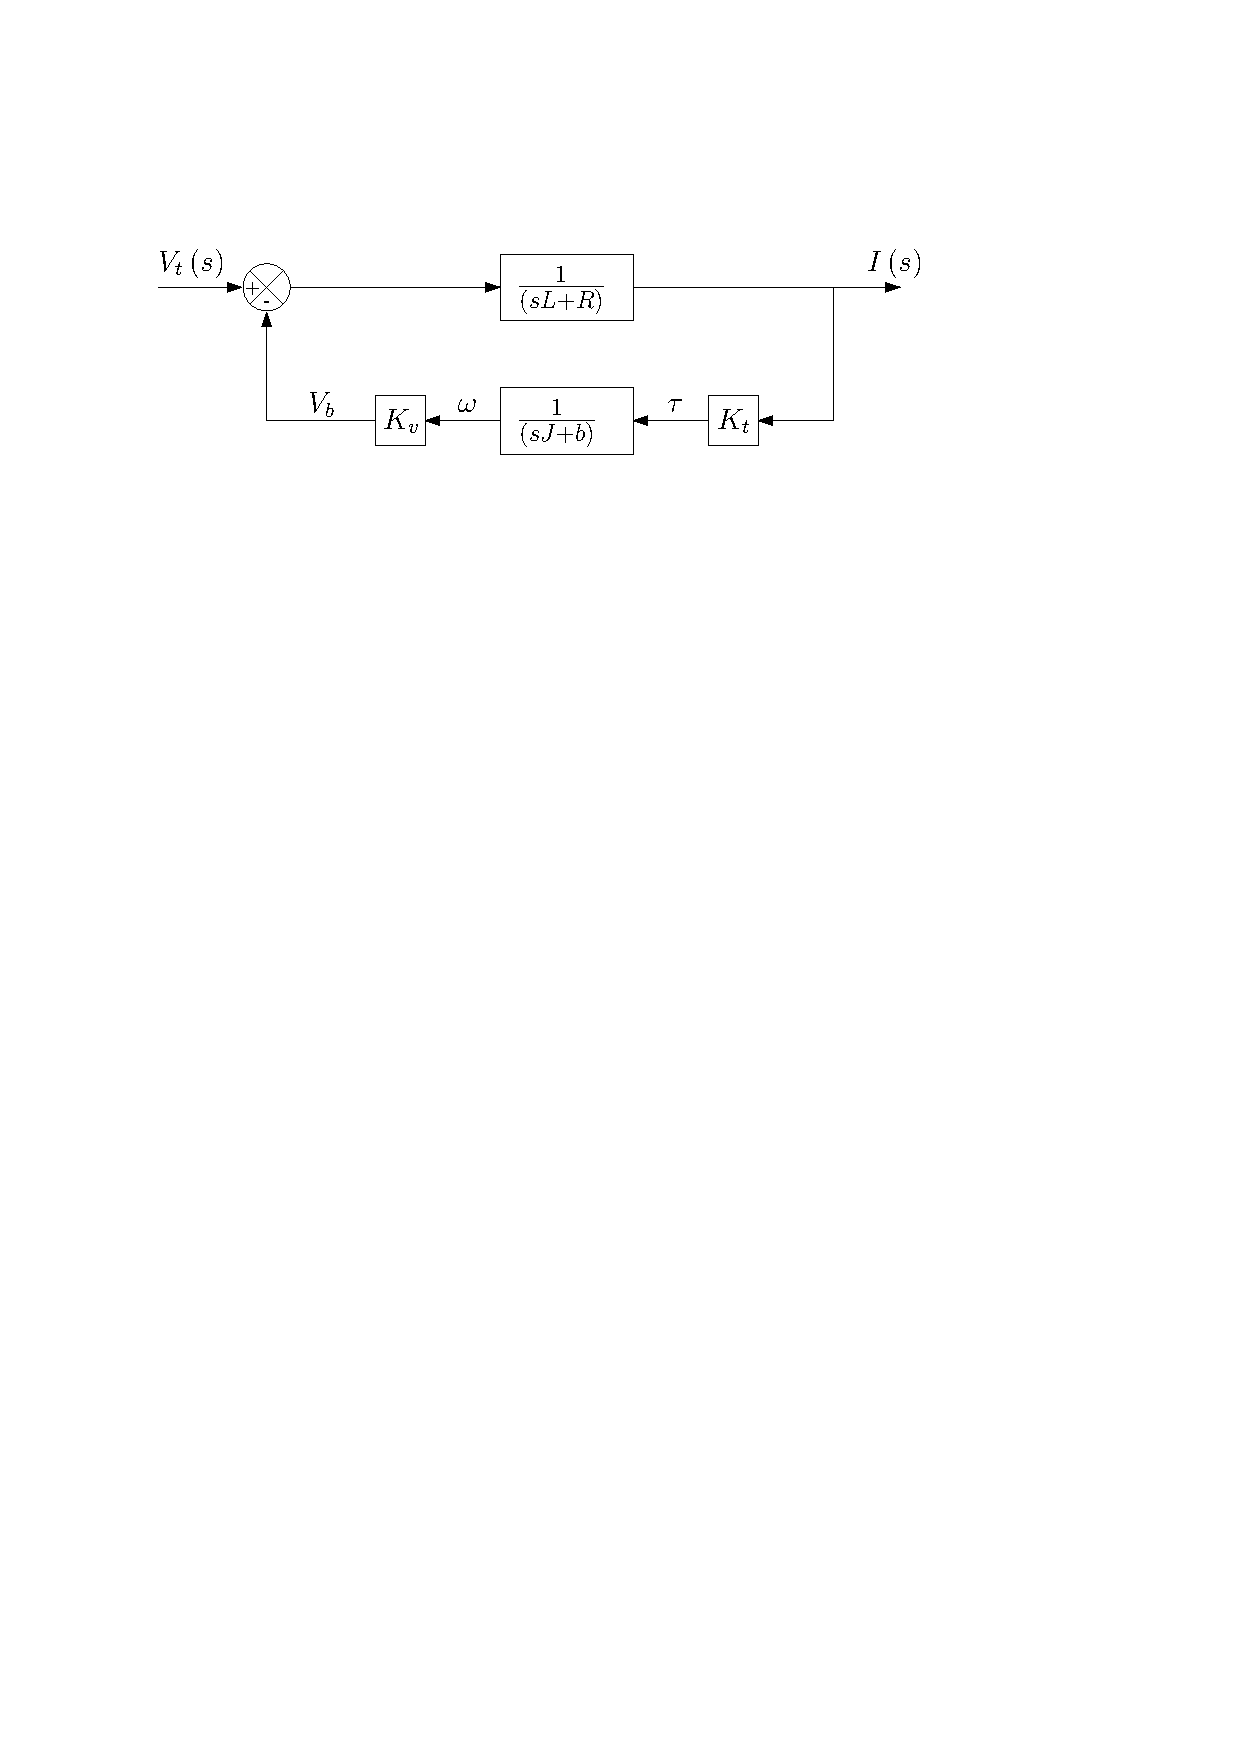
\includegraphics{dc_motor_transfer_fn}	
\caption{Motor transfer function}
\label{fig:dc_motor_transfer_fn}
\end{figure}


The combined transfer function is as follows:

\begin{align}
\frac{I\left(s\right)}{V\left(s\right)} &= \frac{sJ + b}{(sL + R)\cdot(sJ + b) + K_t \cdot K_v} \label{eq:motor_plant_transfer_fn} \\
\nonumber \\
\text{where,} \nonumber \\
I(s) &= \text{winding current} \nonumber \\
V(s) &= \text{terminal voltage} \nonumber \\
K_t &= \text{torque constant} \nonumber \\
K_v &= \text{back emf constant} \nonumber \\
J &= \text{rotor inertia} \nonumber\\
b &= \text{rotor friction-damping} \nonumber \\
L &= \text{winding inductance} \nonumber \\
R &= \text{winding resistance} \nonumber \\
V_b &= \text{back emf} \nonumber \\
\omega &= \text{rotor angular velocity} \nonumber \\
\tau &= \text{torque} \nonumber
\end{align}

Equation \ref{eq:motor_plant_transfer_fn} represents the plant dynamics for the controller that we wish to design.

\section{Motor Controller Design and Analysis}	\label{sec:motor_control_analysis}

The winding current is controlled by applying an appropriate pulse-width-modulated (PWM) voltage ($V_t$) at the motor terminals. The duty cycle of the PWM is calculated by a PI control loop using the current sense as feedback. We shall consider the load disturbance ($d$) and measurement noise ($n$) to analyze the disturbance rejection and noise sensitivity of the controller. We shall look at the bode plots and step responses of the gang of four transfer functions \cite{gang_of_four}.

\begin{figure}
\centering
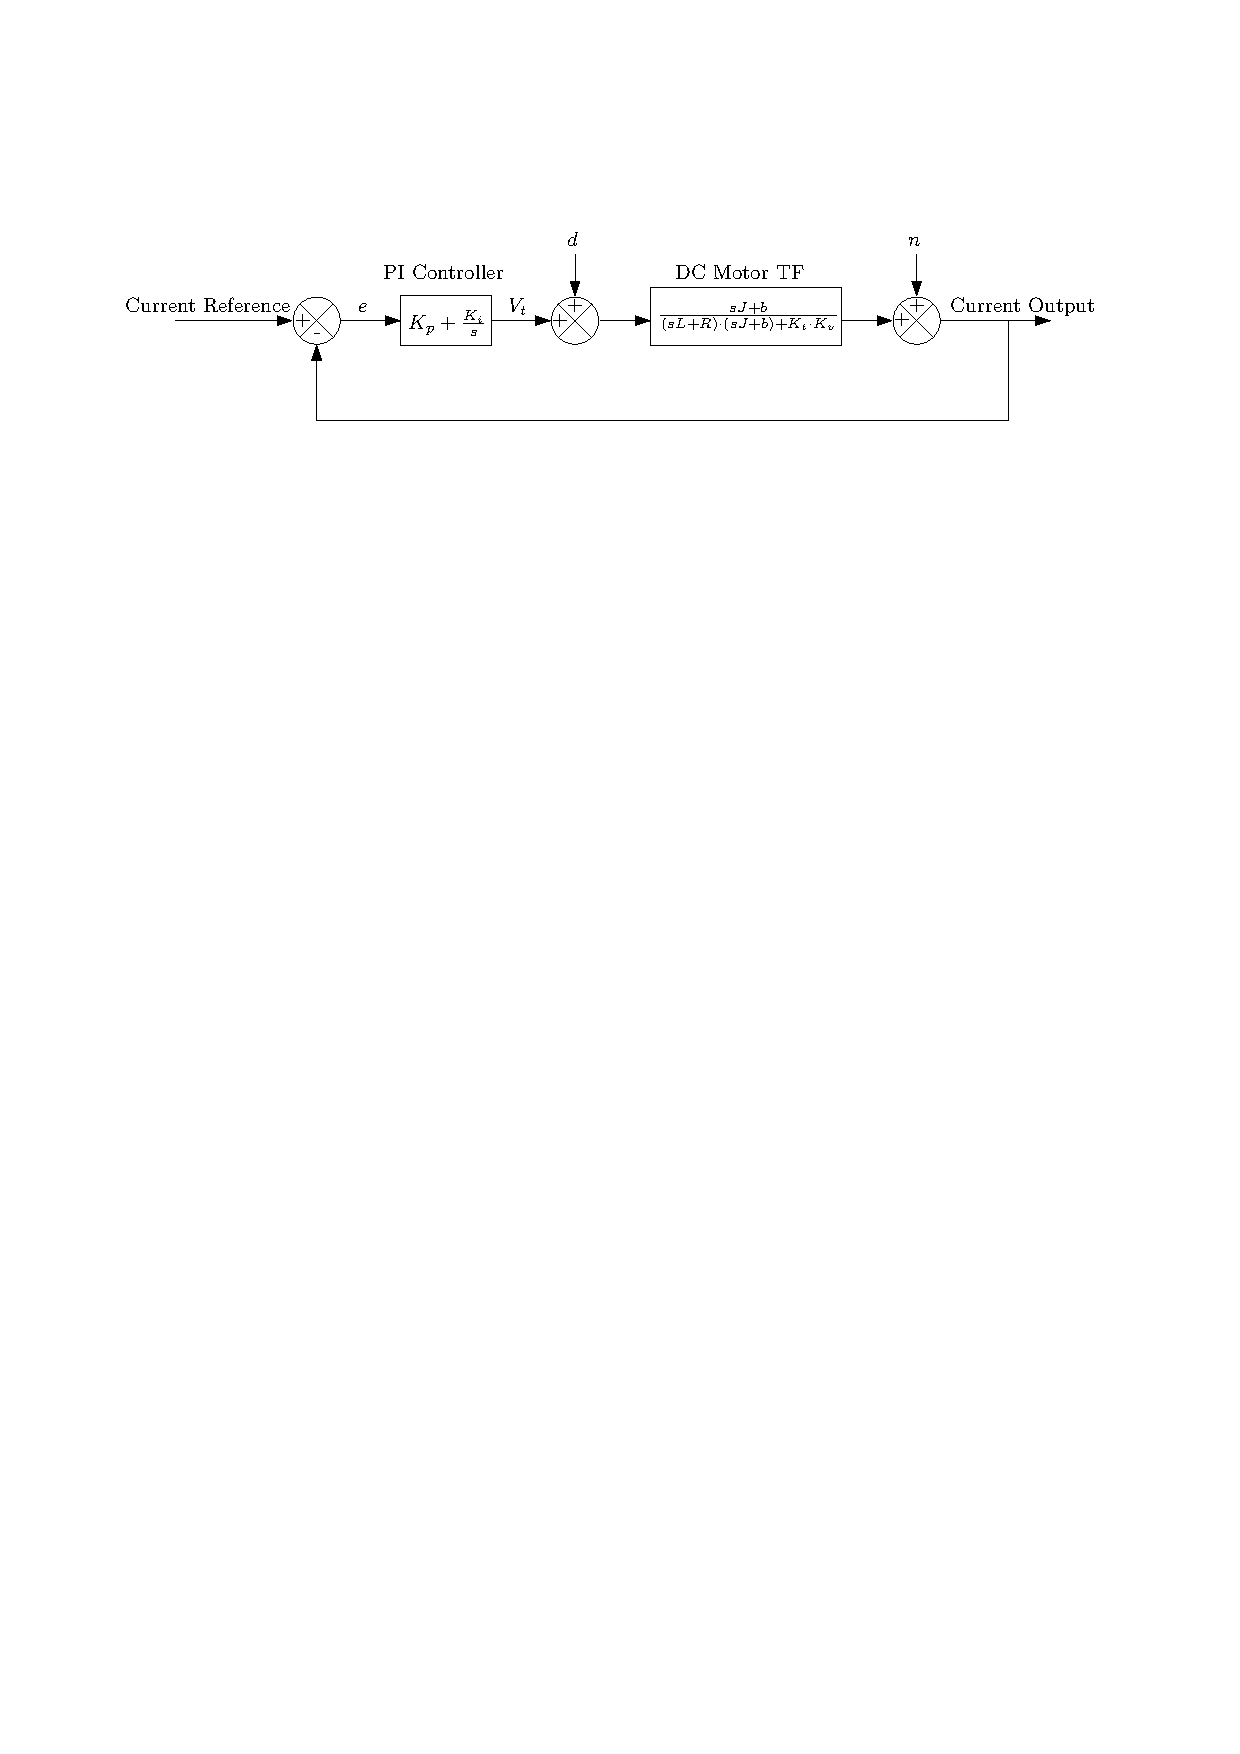
\includegraphics{motor_control_diagram}	
\caption{Current control diagram}
\label{fig:motor_control_diagram}
\end{figure}

\subsection{Plant Characteristics}
Figures \ref{fig:motor_plant_bode} and \ref{fig:motor_plant_step_response} show the plant characteristics without the influence of a controller.
\subsubsection{Transfer Function}
\begin{equation}
\frac{I(s)}{V(s)} = \frac{1.2e-08 s + 0.0151}{2.76e-11 s^2 + 3.476e-05 s + 1.688}
\end{equation}

\begin{figure}[h]
\centering
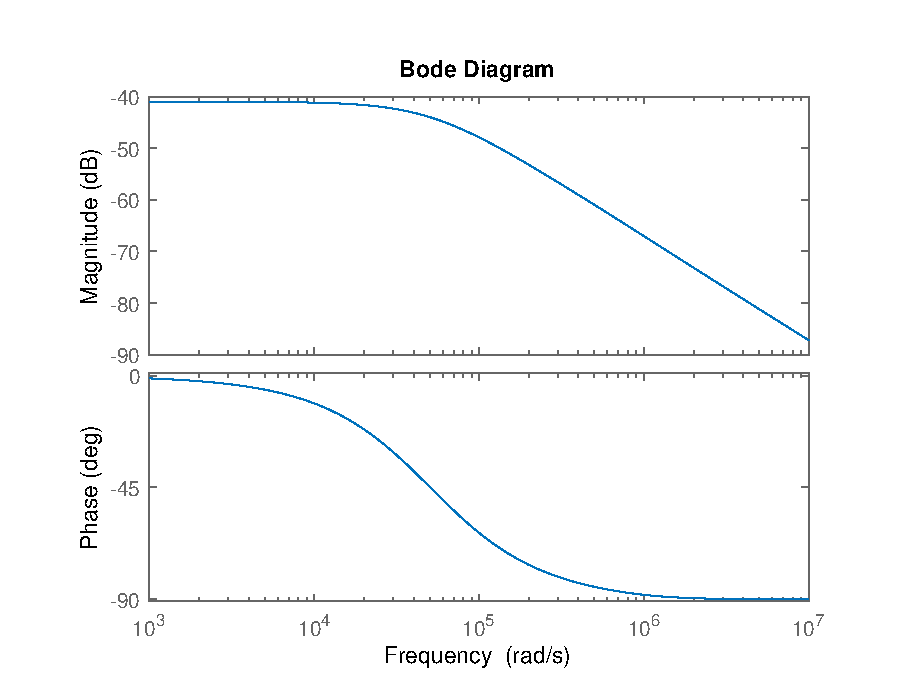
\includegraphics[scale=0.6]{motor_plant_bode}	
\caption{Bode plot of the motor transfer function}
\label{fig:motor_plant_bode}
\end{figure}

\begin{figure}[h]
\centering
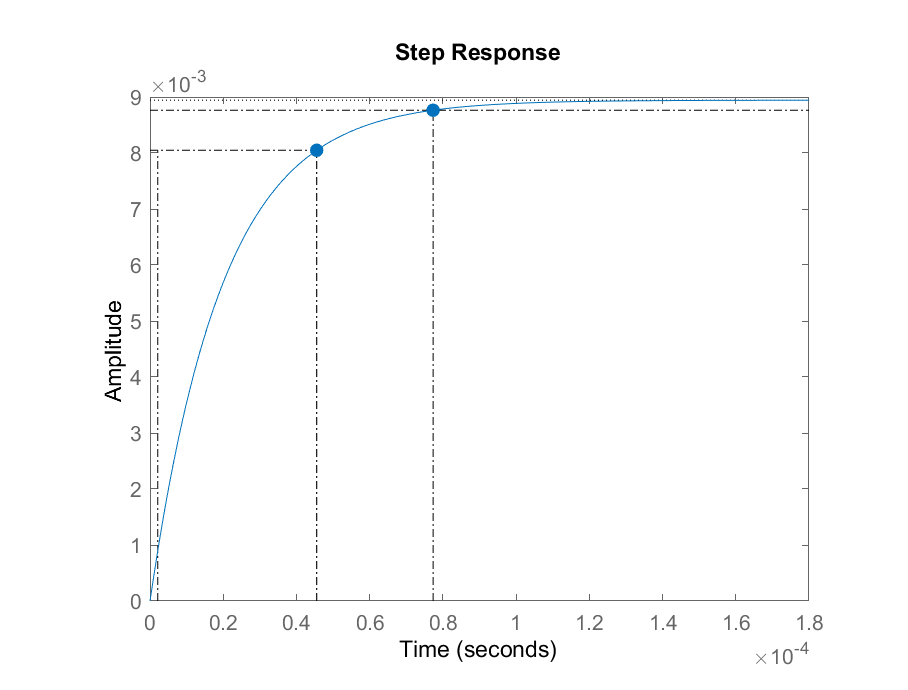
\includegraphics[scale=0.6]{motor_plant_step_response}	
\caption{Step response of the motor transfer function. Rise time = $8e-3$ seconds, settling time = $8.8e-3$ seconds}
\label{fig:motor_plant_step_response}
\end{figure}

\subsection{Closed Loop Characteristics}
Figures \ref{fig:motor_closed_loop_bode} and \ref{fig:motor_closed_loop_step_response} show the closed loop characteristics with PI control loop.
\subsubsection{Transfer Function}
\begin{equation}
\frac{I(s)}{I_{ref}(s)} = \frac{1.543e-17 s^5 + 3.962e-11 s^4 + 2.735e-05 s^3 + 2.47 s^2 + 5.999e04 s}{7.618e-22 s^6 + 1.934e-15 s^5 + 1.341e-09 s^4 + 1.447e-4 s^3 + 5.321 s^2 + 5.999e04 s}
\end{equation}

\begin{figure}[h]
\centering
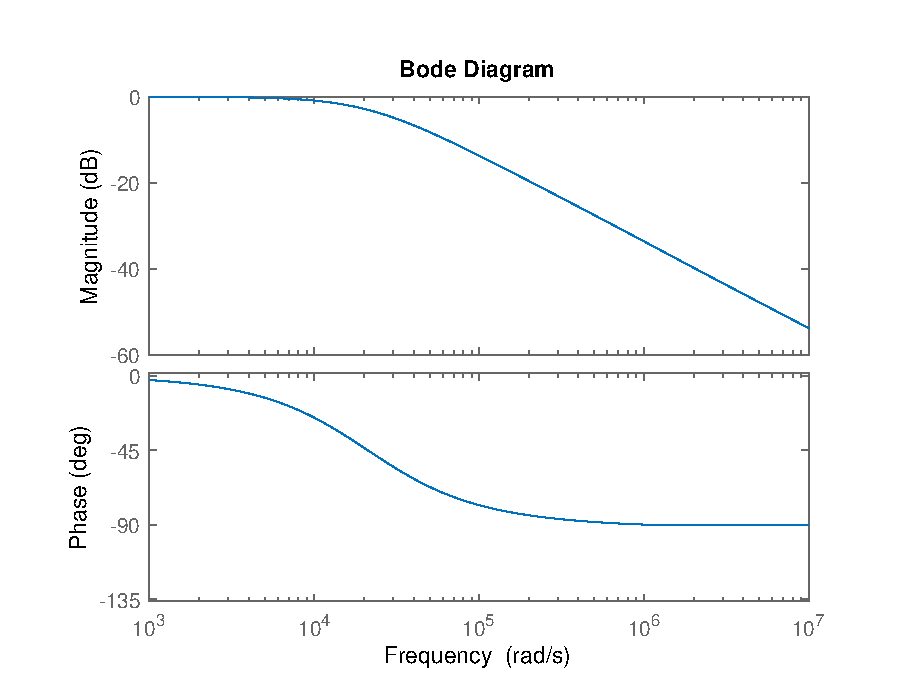
\includegraphics[scale=0.6]{motor_closed_loop_bode}	
\caption{Bode plot of the closed loop transfer function}
\label{fig:motor_closed_loop_bode}
\end{figure}

\begin{figure}[h]
\centering
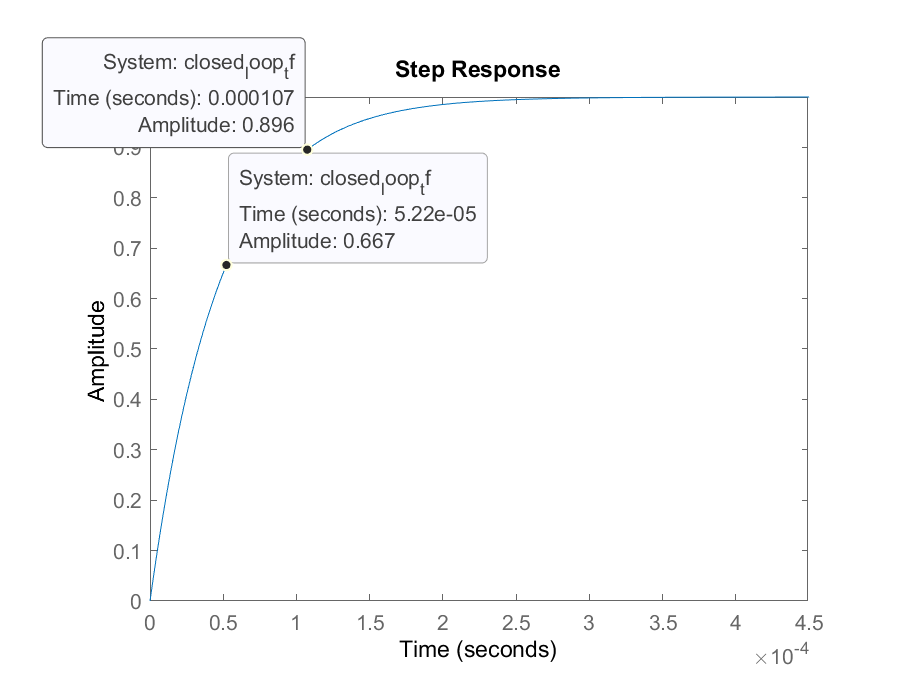
\includegraphics[scale=0.6]{motor_closed_loop_step_response}	
\caption{Step response of the closed loop transfer function. Time to reach 66\% = $5.22e-5$ seconds, time to reach 90\% = $1.07e-4$ seconds }
\label{fig:motor_closed_loop_step_response}
\end{figure}


\subsection{Noise Sensitivity Characteristics}
Figures \ref{fig:motor_noise_sensitivity_bode} and \ref{fig:motor_noise_sensitivity_step_response} show the noise sensitivity characteristics. We can see that low frequency noise is well-attenuated, and a step in noise is short-lived (about $1e-4$ seconds).
\subsubsection{Transfer Function}
\begin{equation}
\frac{I(s)}{N(s)} = \frac{2.76e-11 s^3 + 3.476e-05 s^2 + 1.688 s}{2.76e-11 s^3 + 3.532e-05 s^2 + 2.42 s + 3.553e04}
\end{equation}

\begin{figure}[h]
\centering
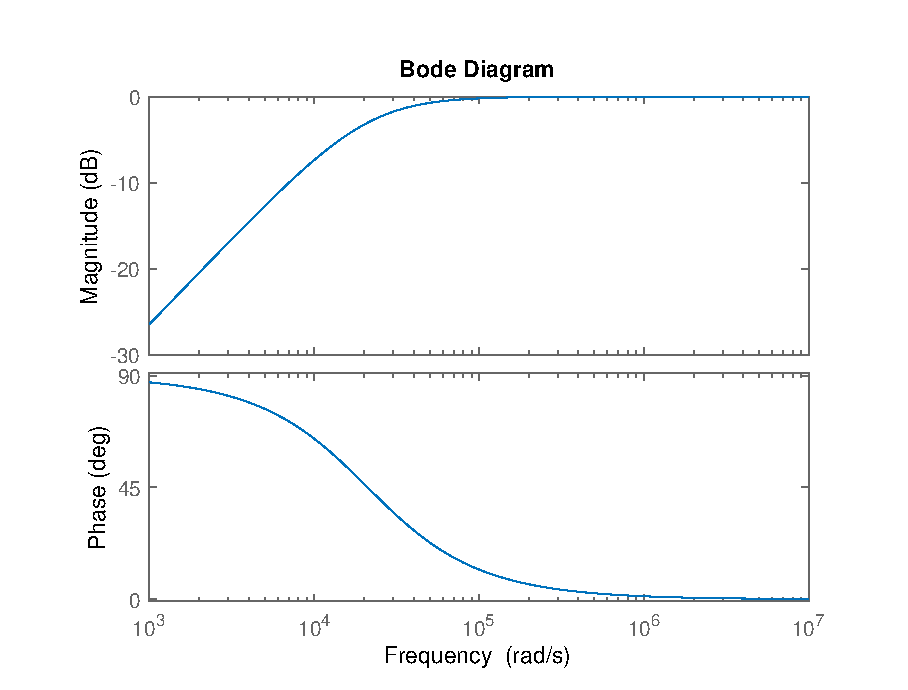
\includegraphics[scale=0.6]{motor_noise_sensitivity_bode}	
\caption{Bode plot of the noise sensitivity transfer function}
\label{fig:motor_noise_sensitivity_bode}
\end{figure}

\begin{figure}[h]
\centering
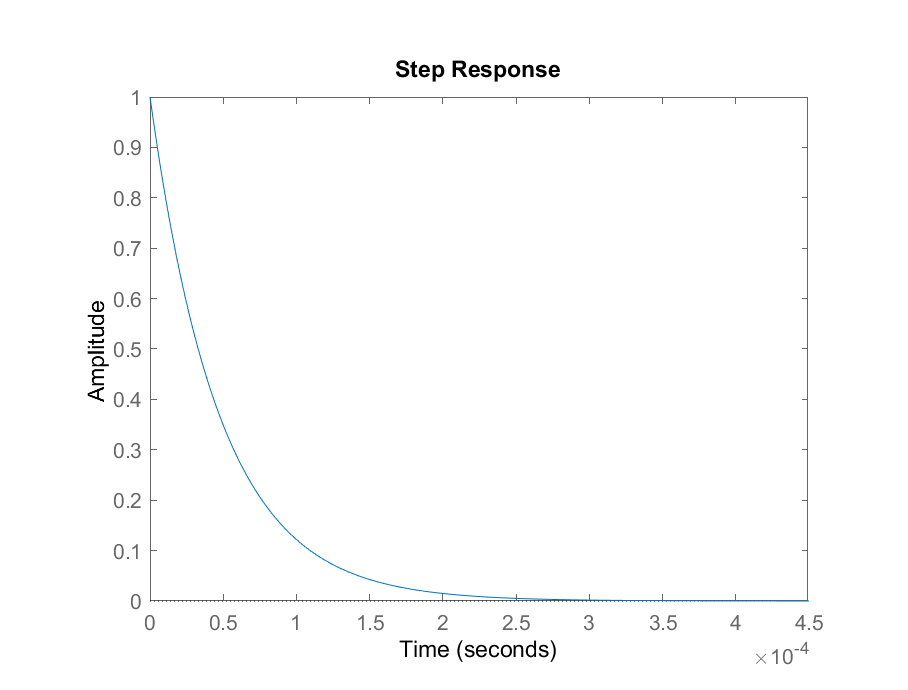
\includegraphics[scale=0.6]{motor_noise_sensitivity_step_response}	
\caption{Step response of the noise sensitivity transfer function}
\label{fig:motor_noise_sensitivity_step_response}
\end{figure}







\bibliographystyle{plain} 
\bibliography{furuta_bib}


\end{document}
